In order to test the accuracy and capability of the Sparrow v4 wireless sensor nodes, we 
have built a shake table in order to simulate the movements of a building during an earthquake.
The purpose of the experiment is to see if the Sparrow v4 nodes can detect the main waves which 
are felt during an earthquake, P-waves and S-waves.

P-waves stands for Primary Waves and is a type of seismic wave produced when an earthquake occurs.
Amongst seismic waves, it has the highest velocity, making it the first wave which is recorded by 
conventional seismographs. This wave is formed by alternating compressions and rarefactions of the 
material and its mode of propagation is always longitudinal. The other type of wave which can be 
recorded during an earthquake is the S-wave which stands for secondary or shear wave. S-waves move 
in a transversal manner through the body of an object, thus resulting in motion which is perpendicular 
to the direction of wave propagation. 

The experimental setup tries to emulate the effects of these waves on a tall building which has Sparrow v4 
nodes mounted on its sides. The purpose of the experiment is to see how accurate the data harvested by the 
IMU is and how the amplitude of the movement varies from floor to floor.

\begin{figure}[ht] \centering
  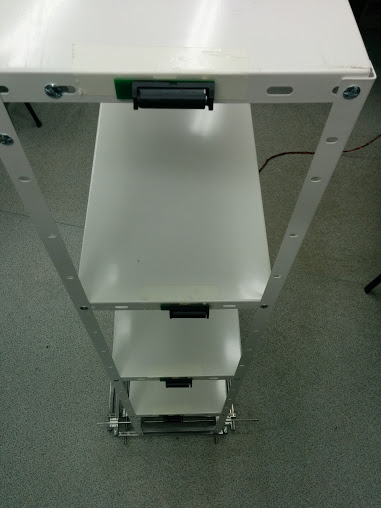
\includegraphics[width=0.5\textwidth]{img/mounted-sparrow-nodes.jpg}
  \caption{SparrowE wireless sensor nodes mounted on the experimental rig}
\end{figure}

In order to perform the experiment, an experimental rig was built. This rig uses a movable frame as its base, 
and a tall, layered shelf mounted on top of it. The frame is composed of two individual planes which are moved 
individually by two DC motors. One plane produces left-right movement, while the other moves the shelf forward and 
backward. The planes are connected to the corresponding motor via a crank whose length can be adjusted, thus giving the 
ability to control the amplitude of the movement. Smaller amplitudes will result in sudden and violent shakes while 
higher amplitudes will allow the shelf to sway more. The schematic of the movable frame is presented below:

\begin{figure}[ht] \centering
  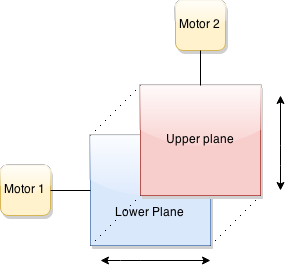
\includegraphics[width=0.5\textwidth]{img/experimental-rig.png}
  \caption{Experimental rig moving frame diagram}
\end{figure}

During the experiment, we harvest the accelerometer data from the Sparrow v4 sensors' IMU at various movement speeds.
The movement speed is controlled by the supply voltage on the motors. The supply values we chose for the experiment 
are 2V, 4V, 7V and 12V, simulating low, medium, high and extremely high vibrations.
